%Capitulo "Elastodinamica"
%
\chapter{Equilibrium Equations}

\section{General Equilibrium Equations}
In this section we develop the incremental equations needed in a general non-linear problem.  First, geometric non-linearities valid for any stress-strain pair are considered.  Second, focus is shifted towards the particular case of the Second Piola-Kirchoff-Green Lagrange Strain pair.

Let   represent the current (deformed) configuration of a deformable medium with equilibrium equations and boundary conditions

\begin{equation}
{\sigma _{ij,j}} + {f_i} = 0	 
\end{equation}			

\begin{equation}
{t_i} = {\sigma _{ij}}{\hat n_j}
\end{equation}	 		

where   represents the Cauchy definition of stress (or force per unit of deformed surface) and   the corresponding tractions vector at a surface with outward normal  .  In the equilibrium equations stated in (1) the domain   is unknown which makes the problem inherently non-linear.  On the other hand this equilibrium statement is mathematically indeterminate since 9 unknown stress components must be solved out of 6 field equations.  The indeterminacy is destroyed after the problem is kinematically described and connected to the stress field via constitutive modeling which can involve additional sources of non-linearity.  To summarize the problem is non-linear since the domain   is unknown, this is what we typically call a Geometric Non-linearity and will be reflected in the mathematical description of changes in configuration.



\subsection{Lagrangian description of the equilibrium equations}
The conceptual definition of Cauchy stress is the only one useful for the engineer since it describes forces per unit deformed surface.  This validity is clearly identified in the fact that the equilibrium equations stated in (1) have been formulated in the stressed deformed domain   where the body is in fact in equilibrium.  The difficulty associated with the unknown domain may be dealt with in alternative ways.  In the case of a solid body it is convenient to refer everything to the undeformed or reference configuration (with known domain)   and proceed from there using linearization which corresponds to a Total Lagrangian (TL) approach.  It is then useful to understand the transformation of the problem to   via pullback operations.  This process implies the introduction or consideration of mathematically  defined stress definitions and newly developed kinematic descriptions.  In this section we consider such transformations first from a dynamic point of view and later using thermodynamic principles we address the problem of identifying the proper strain measures.
\begin{figure}[h]
\centering
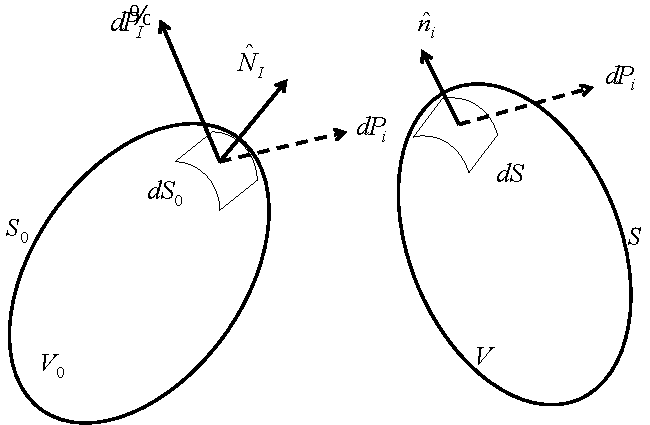
\includegraphics[width=8cm]{img/figure1_2.pdf}
\caption{Definition of the natural domain}
\label{fig:natural domain}
\end{figure}

\subsubsection*{Nanson's formula}
For the treatment that follows it will result useful to consider the relation between oriented differential surface elements in the reference and deformed configurations in the so-called Nanson's formula;

\begin{equation}
\hat{n}_{i}dS=\frac{\rho}{\rho _0}\hat{N}_I f_{Ii}dS_0
\label{nanson}
\end{equation}

\subsubsection*{Lagrangian stress definition}
Let be the differential force associated to the Cauchy physical stress such

\begin{equation}
d{P_i} = {t_i}dS \equiv {\sigma _{ji}}{n_j}dS
\label{diff stress 1}
\end{equation}	 								(3)

Assume that   can also be obtained in the undeformed configuration associated with a new traction definition;

\begin{equation}
d{P_i} = t_i^0d{S_0} \equiv T_{Ii}^0{N_I}d{S_0} \equiv {\sigma _{ji}}{n_j}dS
\label{diff stress 2}	
\end{equation} 						(4)

Using Nanson's formula it is possible to write;

\begin{equation}
T_{Ii}^0{N_I}d{S_0} \equiv {\sigma _{ji}}\frac{{{\rho _0}}}{\rho }{N_I}{f_{Ij}}d{S_0}
\label{equiv}
\end{equation}	 							(5)

Which simplifies into

\begin{equation}
T_{Ii}^0 = \frac{{{\rho _0}}}{\rho }{f_{Ij}}{\sigma _{ji}}
\label{simplified}
\end{equation}	 									(6)

and this is the asymmetric First Piola-Kirchoff stress tensor.

Assume now that there is a pseudo-force in the undeformed configuration   which results from a pullback operation on the physical force  .  Recalling the kinematic connection between the current and undeformed configurations

\begin{equation}
d{X_I} = {f_{Ii}}d{x_i}
\label{pseudo}
\end{equation}	 									(7)

where   is the inverse deformation gradient, we can write for the force and pseudo-force vectors;

\begin{equation}
d{\tilde P_I} = {f_{Ii}}d{P_i}.
\label{for and psefor}
\end{equation}									(8)

Now we can define a tractions vector   in the undeformed configuration and associated with the pseudo-force   like

\begin{equation}
d{\tilde P_I} = {\tilde t_I}d{S_0} \equiv {T_{JI}}{N_J}d{S_0}
\label{unde tracts 1}
\end{equation}	 								(9)

where we have at the same time introduced the associated stress tensor.  It then directly follows that;

\begin{equation}
{T_{JI}}{N_J}d{S_0} = {f_{Ii}}d{P_i} \equiv {f_{Ii}}{\sigma _{ji}}{n_j}dS
\label{unde tracts 2}	 
\end{equation}							(10)

once again using Nanson's formula we can write

\begin{equation}
{T_{JI}}{N_J}d{S_0} = {f_{Ii}}{\sigma _{ji}}\frac{{{\rho _0}}}{\rho }{N_J}{f_{Jj}}d{S_0}
\label{unde tracts 3}
\end{equation}	 							(11)

and

\begin{equation}
{T_{JI}} = \frac{{{\rho _0}}}{\rho }{f_{Jj}}{\sigma _{ji}}{f_{Ii}}
\label{unde tracts 4}
\end{equation}	 								(12)

which corresponds to the symmetric Second Piola-Kirchoff stress tensor.

For the derivations that follow and in the actual computational implementation it will be convenient to have the inverse relationships expressing the Cauchy stress tensor in terms of the First and Second Piola-Kirchoff stress definitions.

Once again recall that   and use the definition found for the first PK stress tensor to write



\section{Equilibrium in Weak Form}
